\section{Introduction}
Mandatory. Questions like: What is the topic of this work, what's the broader context (topic of the proseminar), why is it relevant?

%\begin{itemize}
%    \item History of ensemble learning + papers of people "inventing" it
%    \item Goal of the report
%    \item learning more about bagging + boosting
%    \item get to know most popular types of both methods
%    \item learn how to practically use them
%    \item when to use which technique
%    \item 
%\end{itemize}
% ---------------------------------------------------------------------------- %
\section{Ensemble Learning}

Ensemble learning is an advanced machine learning approach that combines the 
strengths of multiple smaller learning algorithms to improve predictive 
performance. 
The concept behind ensemble learning is analogous to the "wisdom of crowds".
Which describes, that a crowd, on average, makes collectively better decisions,
than any single member of it.

Just as a diverse group of people can provide a more accurate collective decision 
than an individual, in ensemble learning, a combination of learning algorithms
often predicts more accurately than an individual learning algorithm.
This approach is based on the principle that a diverse set of learning algorithms
can capture different patterns or trends in the data, leading to more robust and 
accurate predictions.

To be more precise, ensemble methods use multiple smaller learning algorithms,
which specialize in small aspects of the problem. However, by combining these
algorithms, the ensemble often achieves better predictive performance than 
the used algorithm could achieve alone because they complement each others
strengths and weaknesses.

So the goal of ensemble learning is to achieve a better predictive performance.
Nevertheless, it comes at the cost of increased computational resources for 
training as well as prediction and storage.

Overall, there are many different ensemble methods, such as bagging and boosting, 
which we will go into more detail in this report. However, there are many more 
like stacking and blending.

% TODO: Make image prettier
%\begin{figure}[htbp]
%    \centering
%    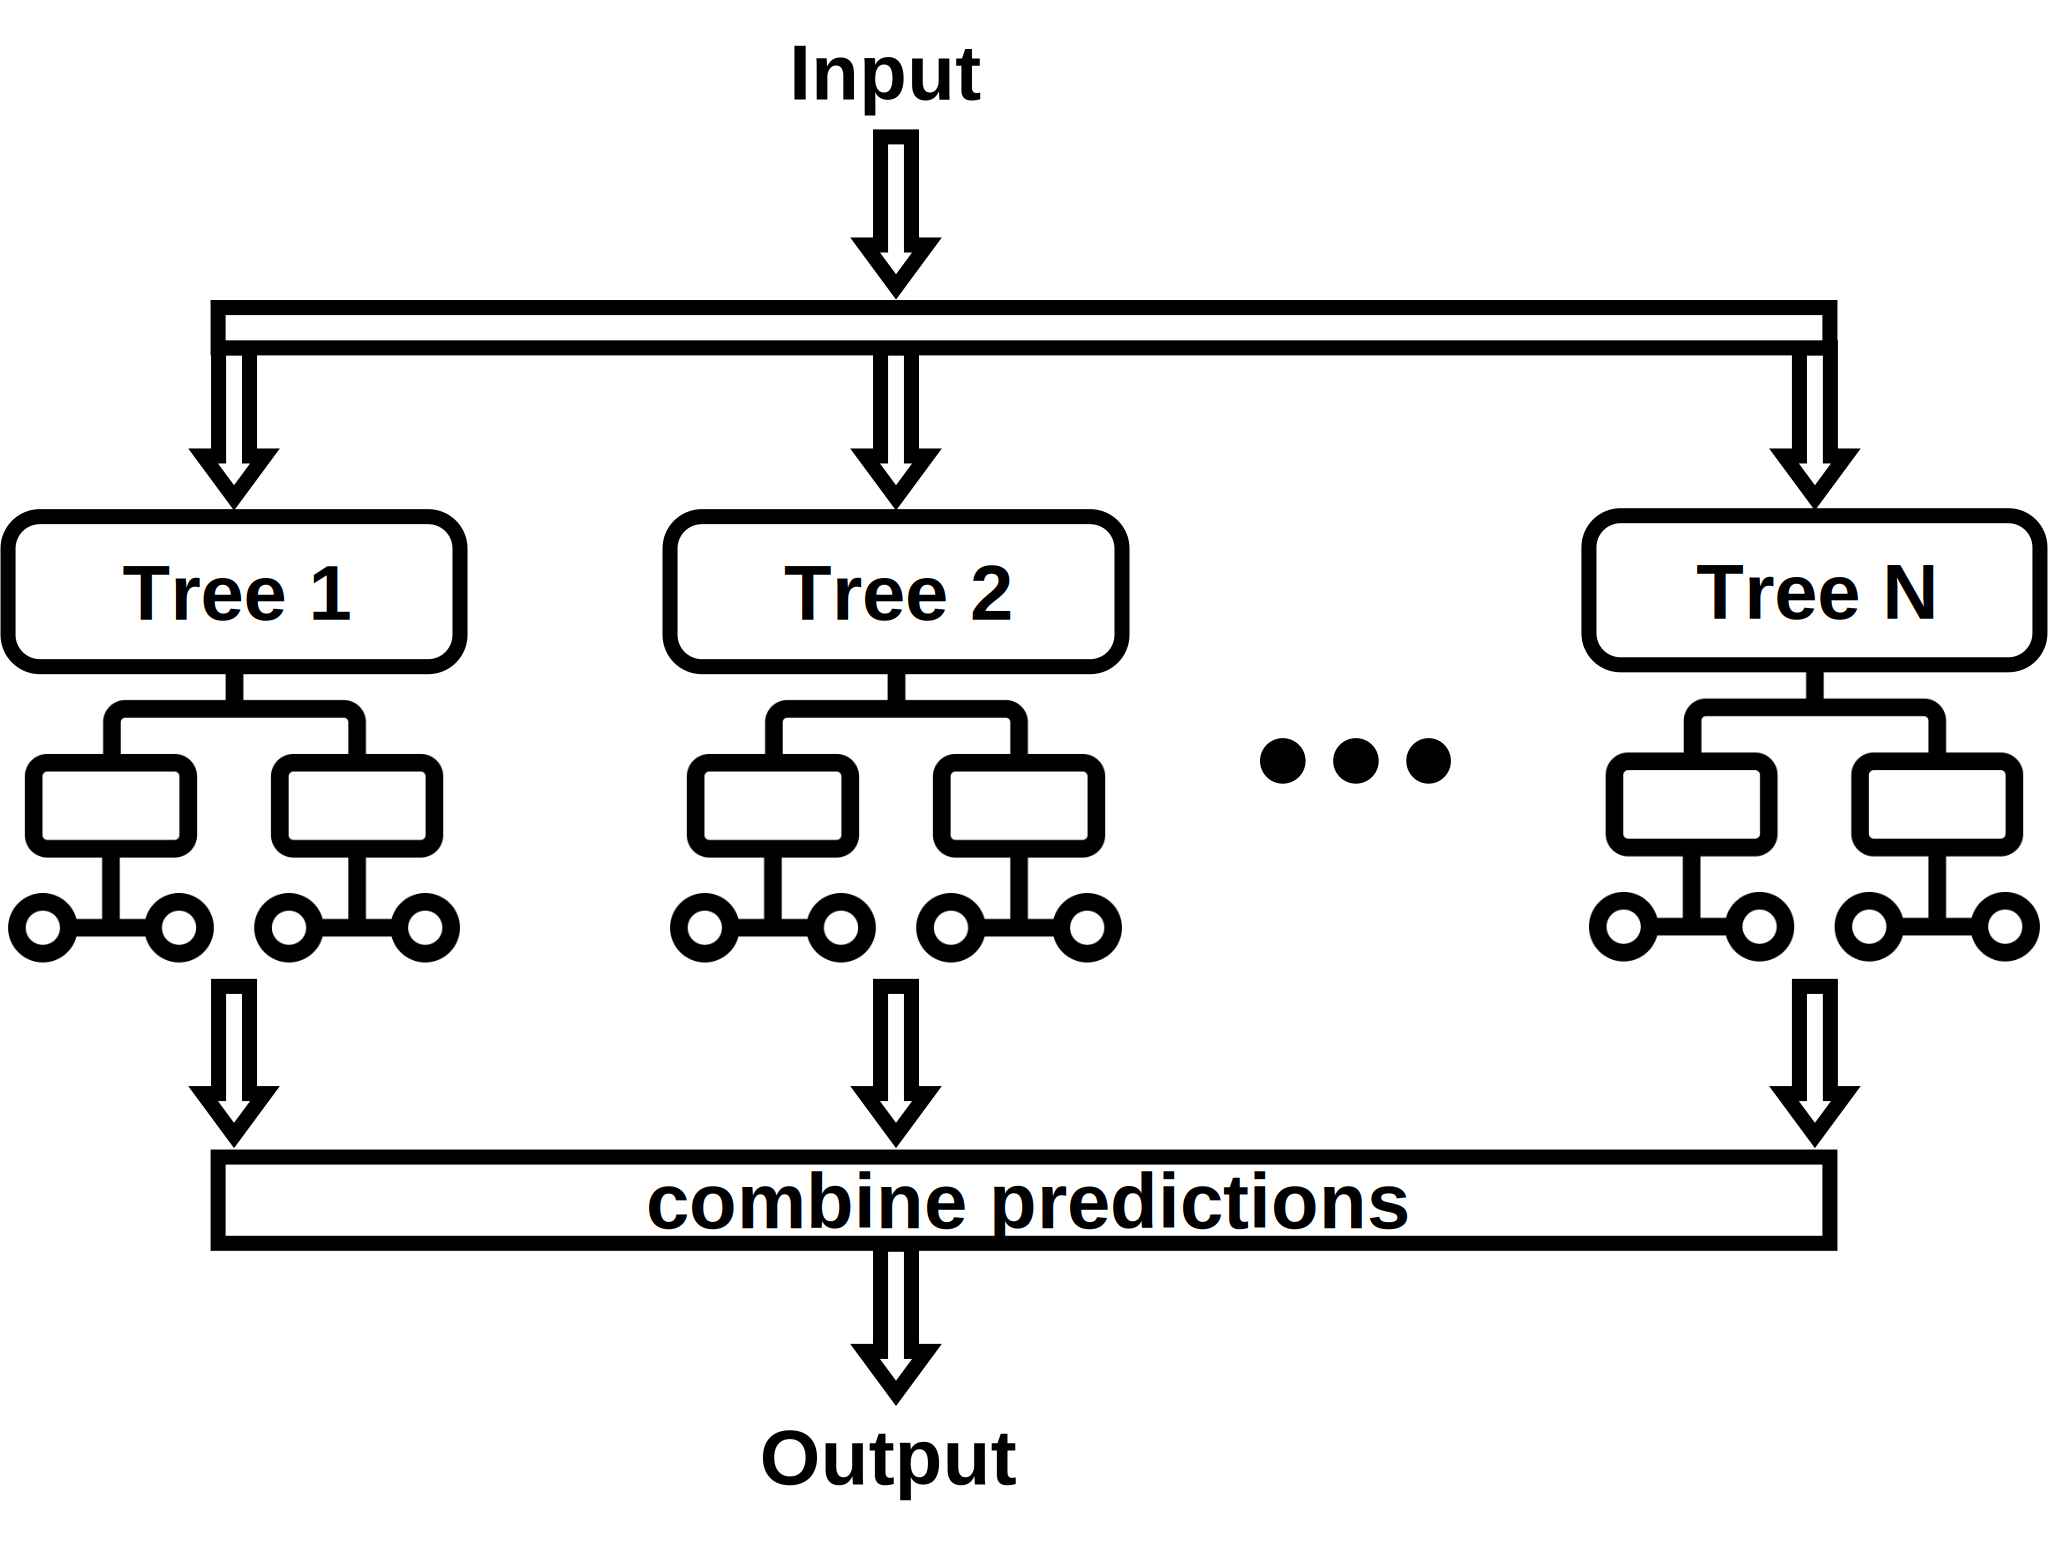
\includegraphics[width=.5\textwidth]{figures/ensemble_method_prediction}
%    \caption{Ensemble learning prediction.}
%\end{figure}

% ---------------------------------------------------------------------------- %
\subsection{Bagging}

% Intro Bagging and Traing
Bootstrap Aggregating, commonly known as bagging, is an ensemble learning method
developed by \citet*{Breiman1996}. The models for the ensemble get trained individually
by using the bootstrapping technique. Bootstrapping involves creating random
subsets of the original training dataset. The subsets are created by drawing 
random data point with replacement and have the same size as the original
training dataset. This means that data points can be chosen more than once and
that some data points might not be in the subset. The models can be trained in
parallel, because of the individual training.


Figure 1 shows how bootstrapping might work on an imaginary dataset. In subset 1
each class is equally distributed. Subset 2 has a focus on the red and orange bubles.
The subset N has a strong focus on blue, however it doesn't even have a single 
orange buble. This will probably mean that the model trained on subset N will be very
good at predicting blue, but not very accurate with orange.

\begin{figure}[htbp]
    \centering
    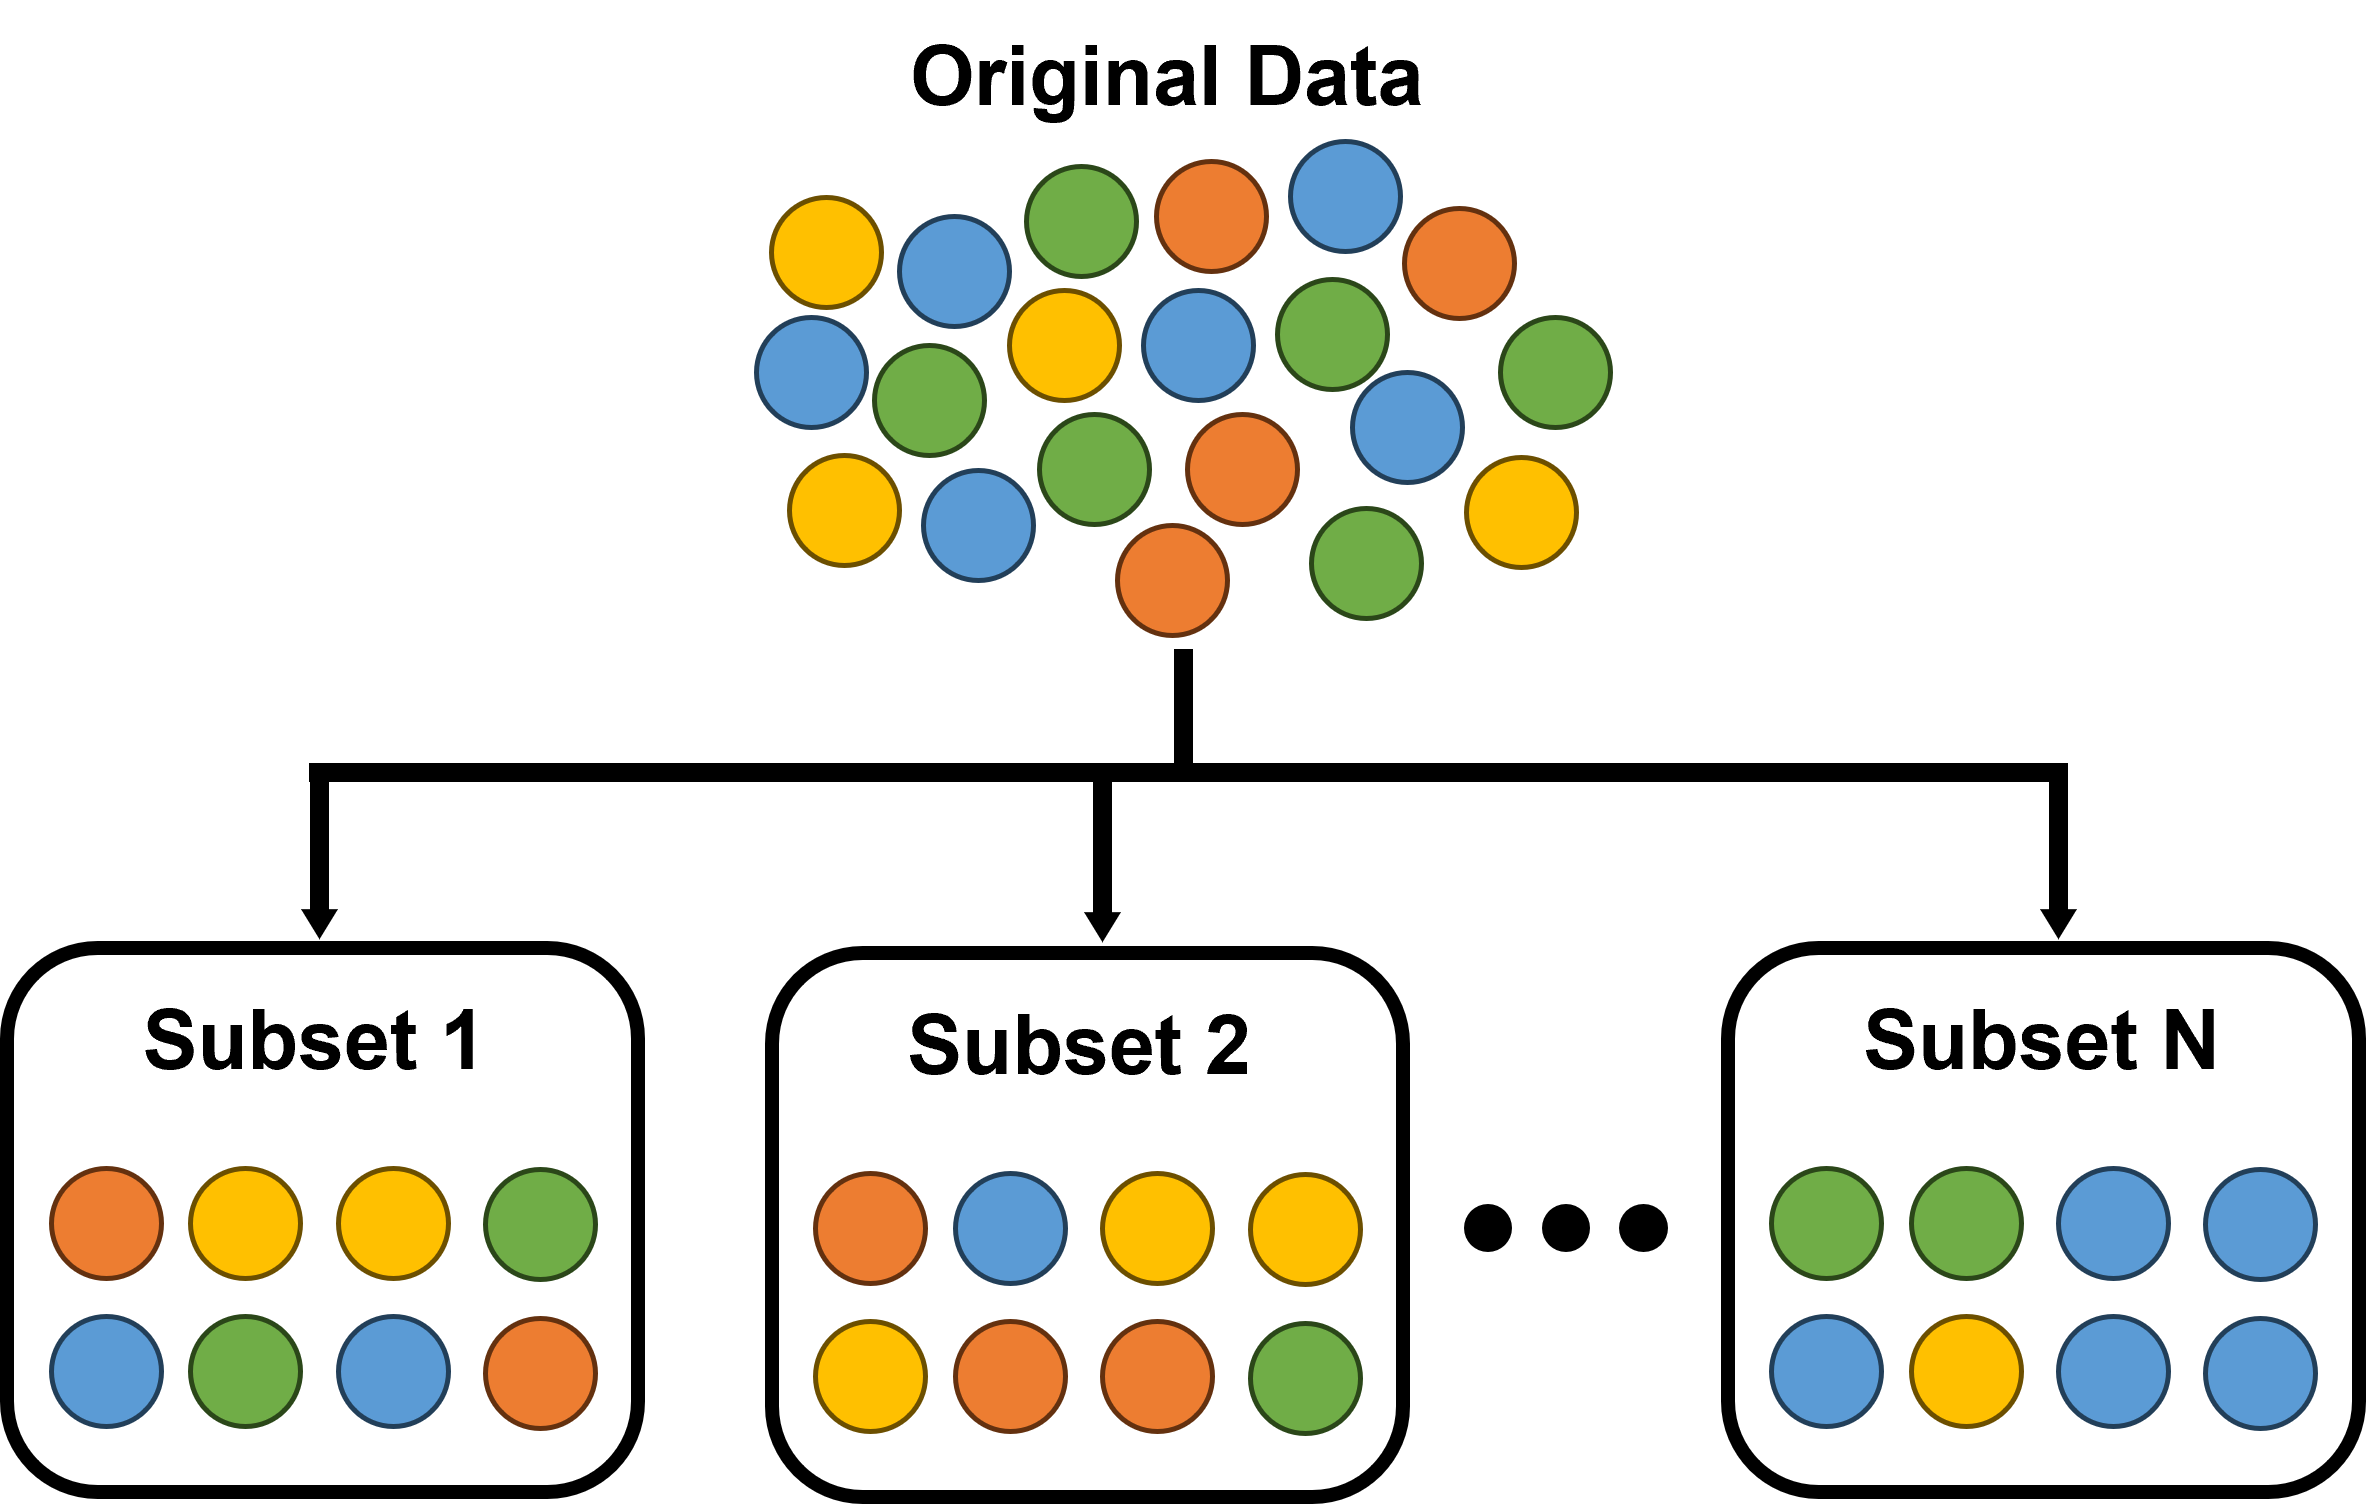
\includegraphics[width=.5\textwidth]{figures/bootstrapping}
    \caption{Creating subsets with bootstrapping.}
\end{figure}

% Prediction Bagging
% TODO: let GPT check
In the bagging ensemble each model makes its prediction independently. Because of
that the predictions of the individual models can be ran in parallel, similar to
the training. Once every model in the ensemble has made their prediction, they get
aggregated to form a final ensemble prediction. The method of aggregation depends
on the problem that is being solved by the bagging ensemble. 
For classification problems a common method is majority voting. Each model votes 
for a particular class. The class that receives the most votes is chosen for the
final ensemble prediciton.
For regression problems the predictions of the individual models are typically 
averaged.

\begin{figure}[htbp]
    \centering
    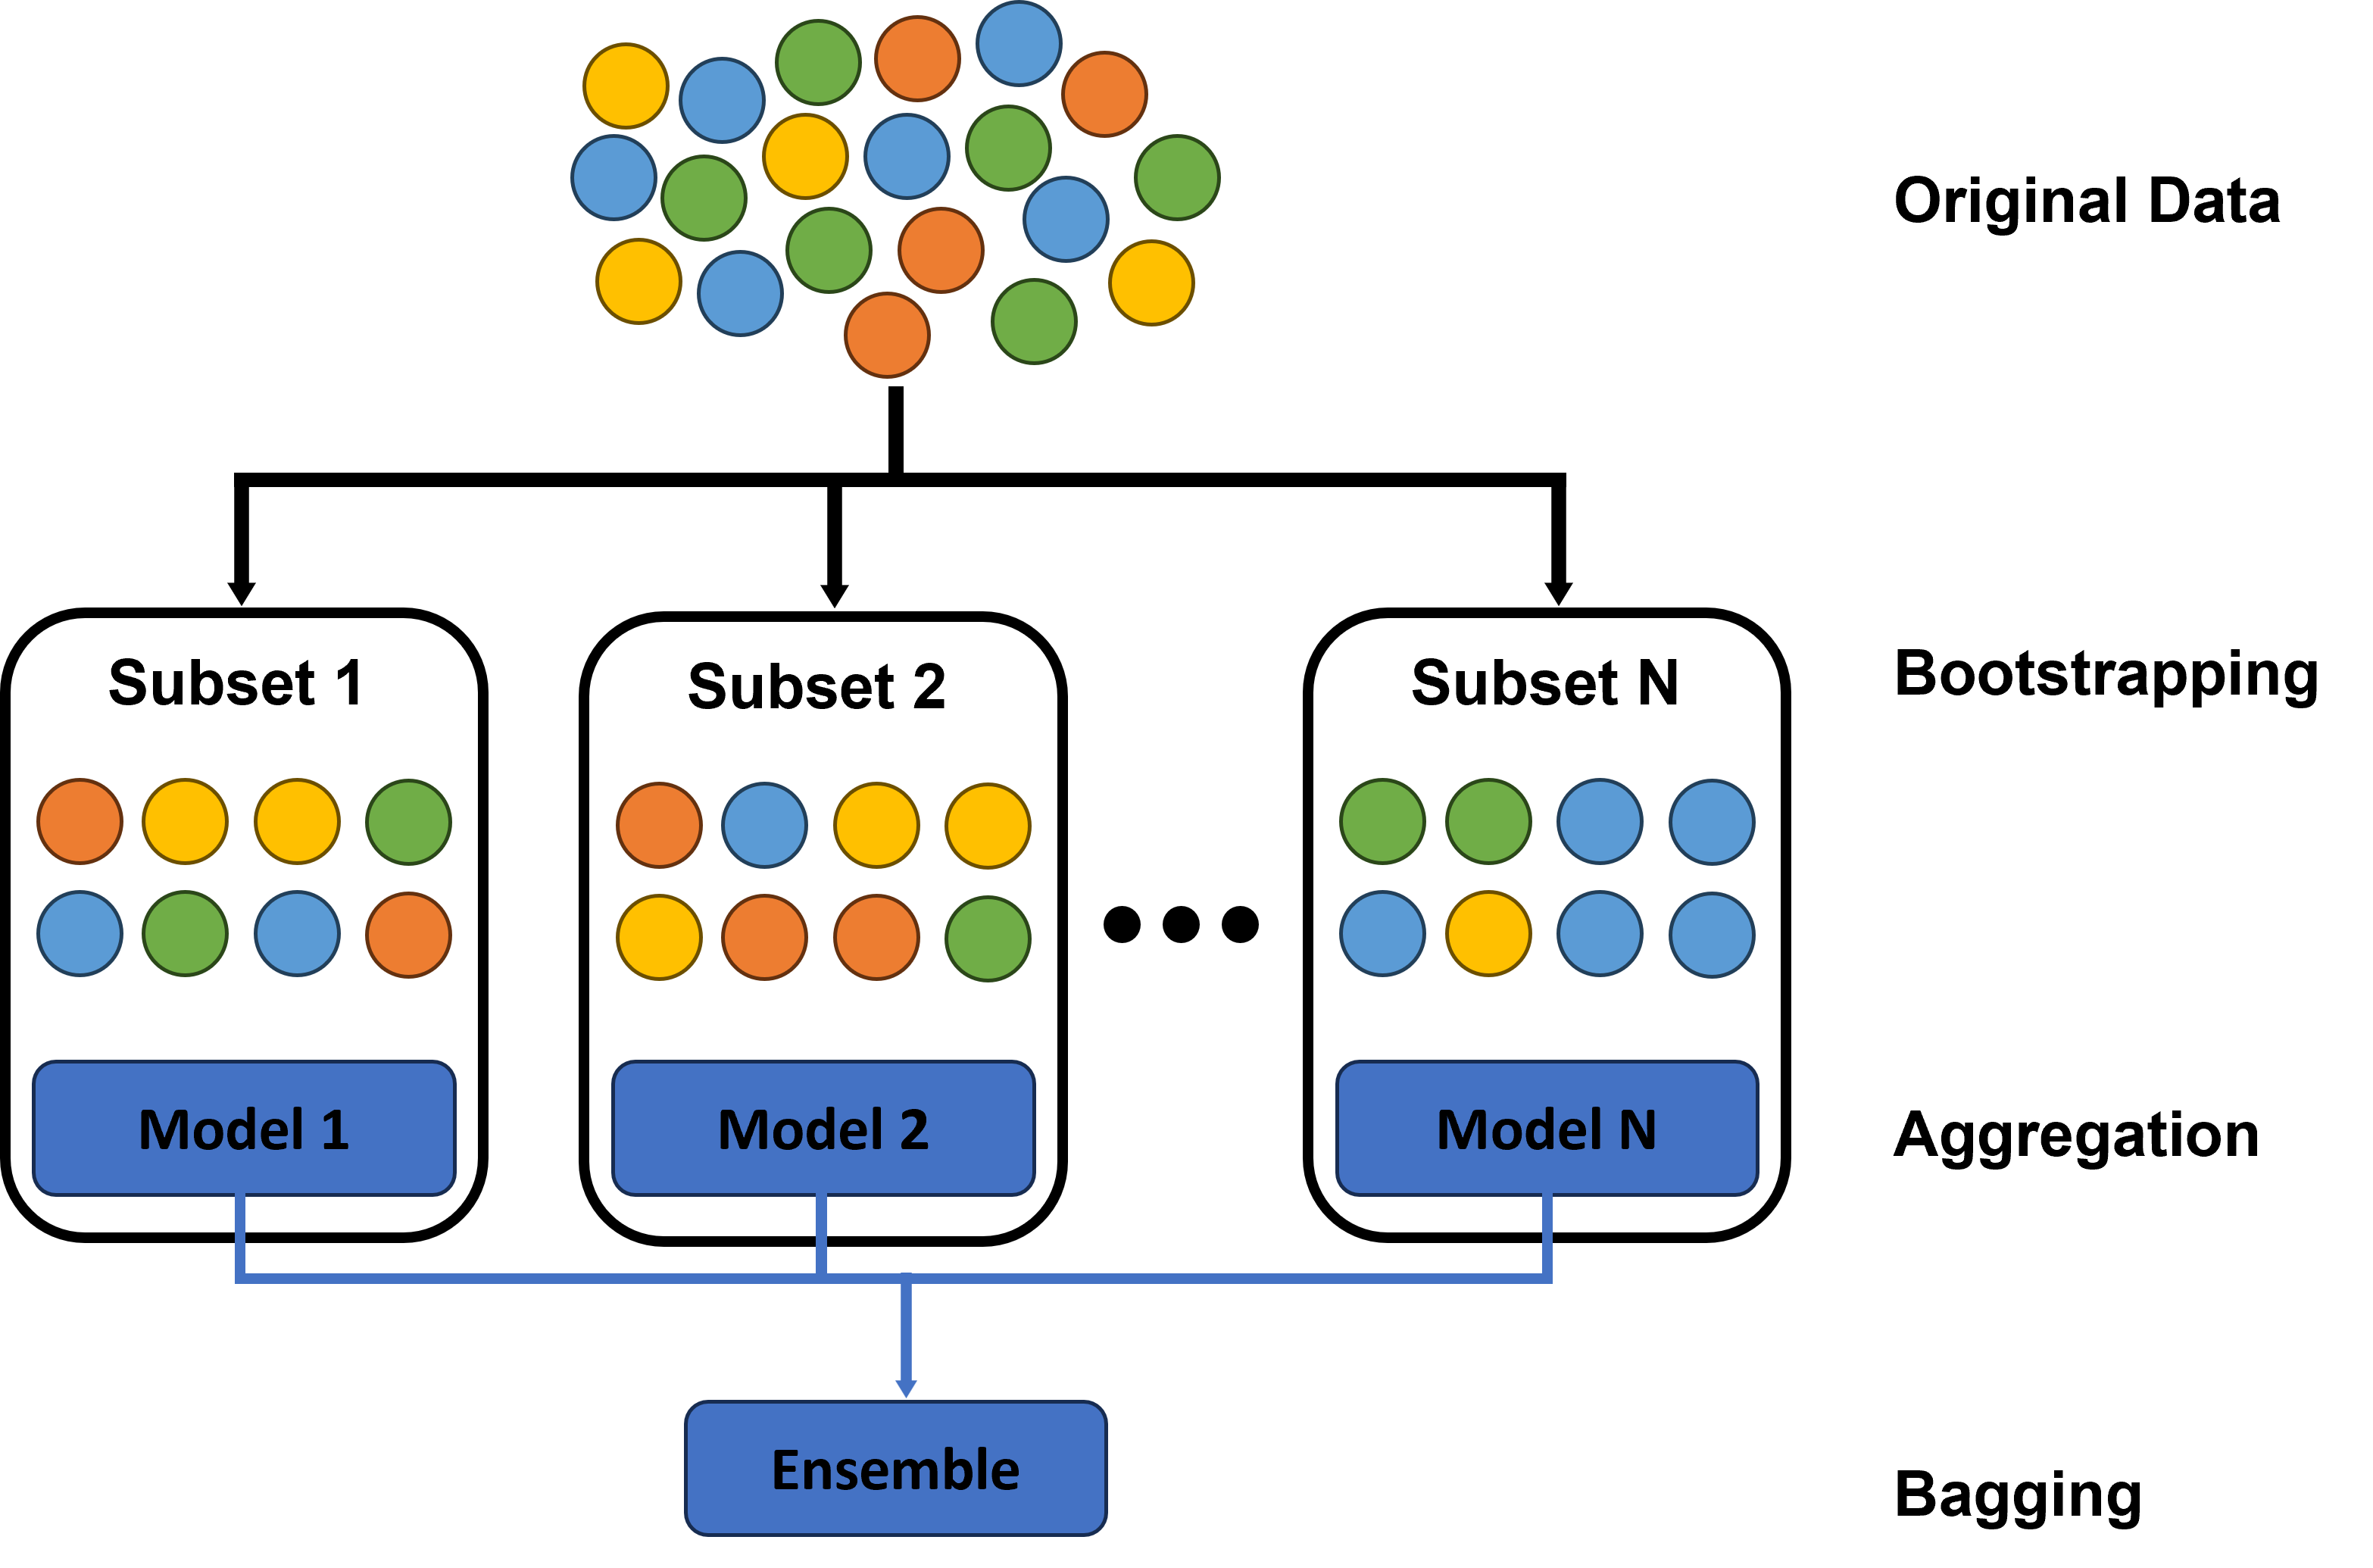
\includegraphics[width=.5\textwidth]{figures/bagging_prediction}
    \caption{Bagging prediction.}
\end{figure}


% When to use bagging (Advantages)
% Utilizing Multiple Cores for Parallel Training / Prediction could be added
Bagging can be particularly effective when using base learning algorithms
that have high variance or tend to overfit quickly. By bootstrapping and 
averaging the predictions the variance gets reduced and potential overfitting
is avoided.
Same goes for unstable learning algorithms, that produce significantly different
results on small changes in the data. Thats why bagging is often used with decision
trees as they tend to be unstable and to have high variance.
Additionally, bagging can be very helpful when dealing with noisy, imbalanced 
datasets or datasets with missing data. The bootstrapping helps to create 
diverse datasets with each class being adequately represented and also averaging
out the noise in combination with aggregation.


% Summary
All in all, bagging can help to reduce variance, prevent overfitting and to built
a more resilient, robust and generalized model.

\subsection{Random Forest}
%\begin{itemize}
%    \item difference to bagging
%\end{itemize}

% TODO: adden wenn noch Platz - \subsection{Out-of-bag}

\subsection{Boosting}
%\begin{itemize}
%    \item Whats the idea behind it?
%    \item How to train boosting? (+ graphic)
%    \item How does the prediction work? (+ graphic)
%    \item when to use it
%    \item advantages and challenges of using it
%\end{itemize}

\subsection{Gradient Boosting}
%\begin{itemize}
%    \item difference to boosting
%\end{itemize}

\subsection{Extreme Gradient Boosting}
%\begin{itemize}
%    \item difference to gradient boosting
%\end{itemize}


% ---------------------------------------------------------------------------- %
\section{Examples}
\subsection{Example 1}
\subsection{Example 2}

% ---------------------------------------------------------------------------- %
\section{Summary and conclusion}
Mandatory. Short summary of the most important aspects of the report.
If possible: What are open challenges?

\begin{itemize}
    \item Bagging vs. Boosting - whats the difference?
\end{itemize}


%\newpage
%\section{\LaTeX Examples}
%As a help to get started with this template. To be deleted for submission.
%\subsection{Citation examples}
%\citet{campbell:2017} define the stages of information processing in a nervous system as: "sensory input, integration, and motor output". \\
%The stages of information processing in a nervous system are defined as: "sensory input, integration, and motor output" \citep{campbell:2017}. 
%
%\subsection{Table example}
%\begin{table}[htbp]
    \centering
    \begin{tabular}{lrl}
    \toprule
    labels   & numbers & annotation \\
    \midrule
    abra     &  1.23   & \textbf{this is important}\\
    cadabra  &  2.34   & this isn't\\
    \bottomrule
    \end{tabular}
    \caption{Some random numbers}
    \label{tab:random}
\end{table}
%
%\subsection{Figure examples}
%This is a png file, it gets blurry when you zoom in:
%\begin{figure}[htbp]
%    \centering
%    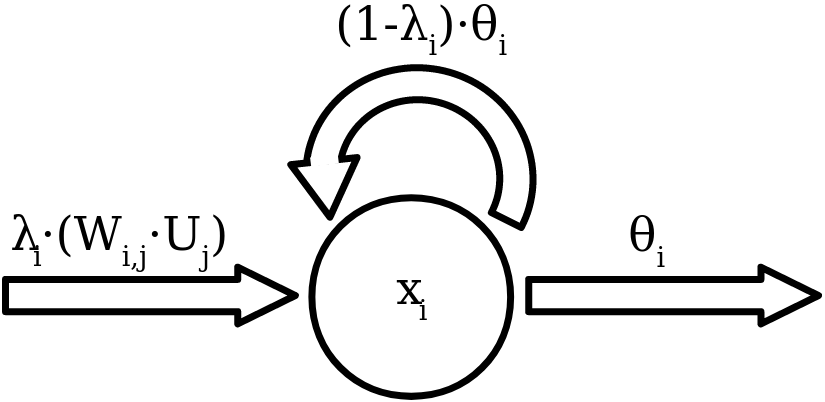
\includegraphics[width=.7\textwidth]{figures/leaky_integration.png}
%    \caption{Symbolic representation of a leaky integrating neuron.}
%    \label{fig:leaky_integration}
%\end{figure}
%
%This is an eps file, it is always sharp:\\
%Notice how the formatting option "[htbp]" allows for the figure to be moved around to page \pageref{fig:activation_function}. Hence, it is best to rather write: The eps file in figure \ref{fig:activation_function} always stays sharp.
%\begin{figure}[htbp]
%    \centering
%    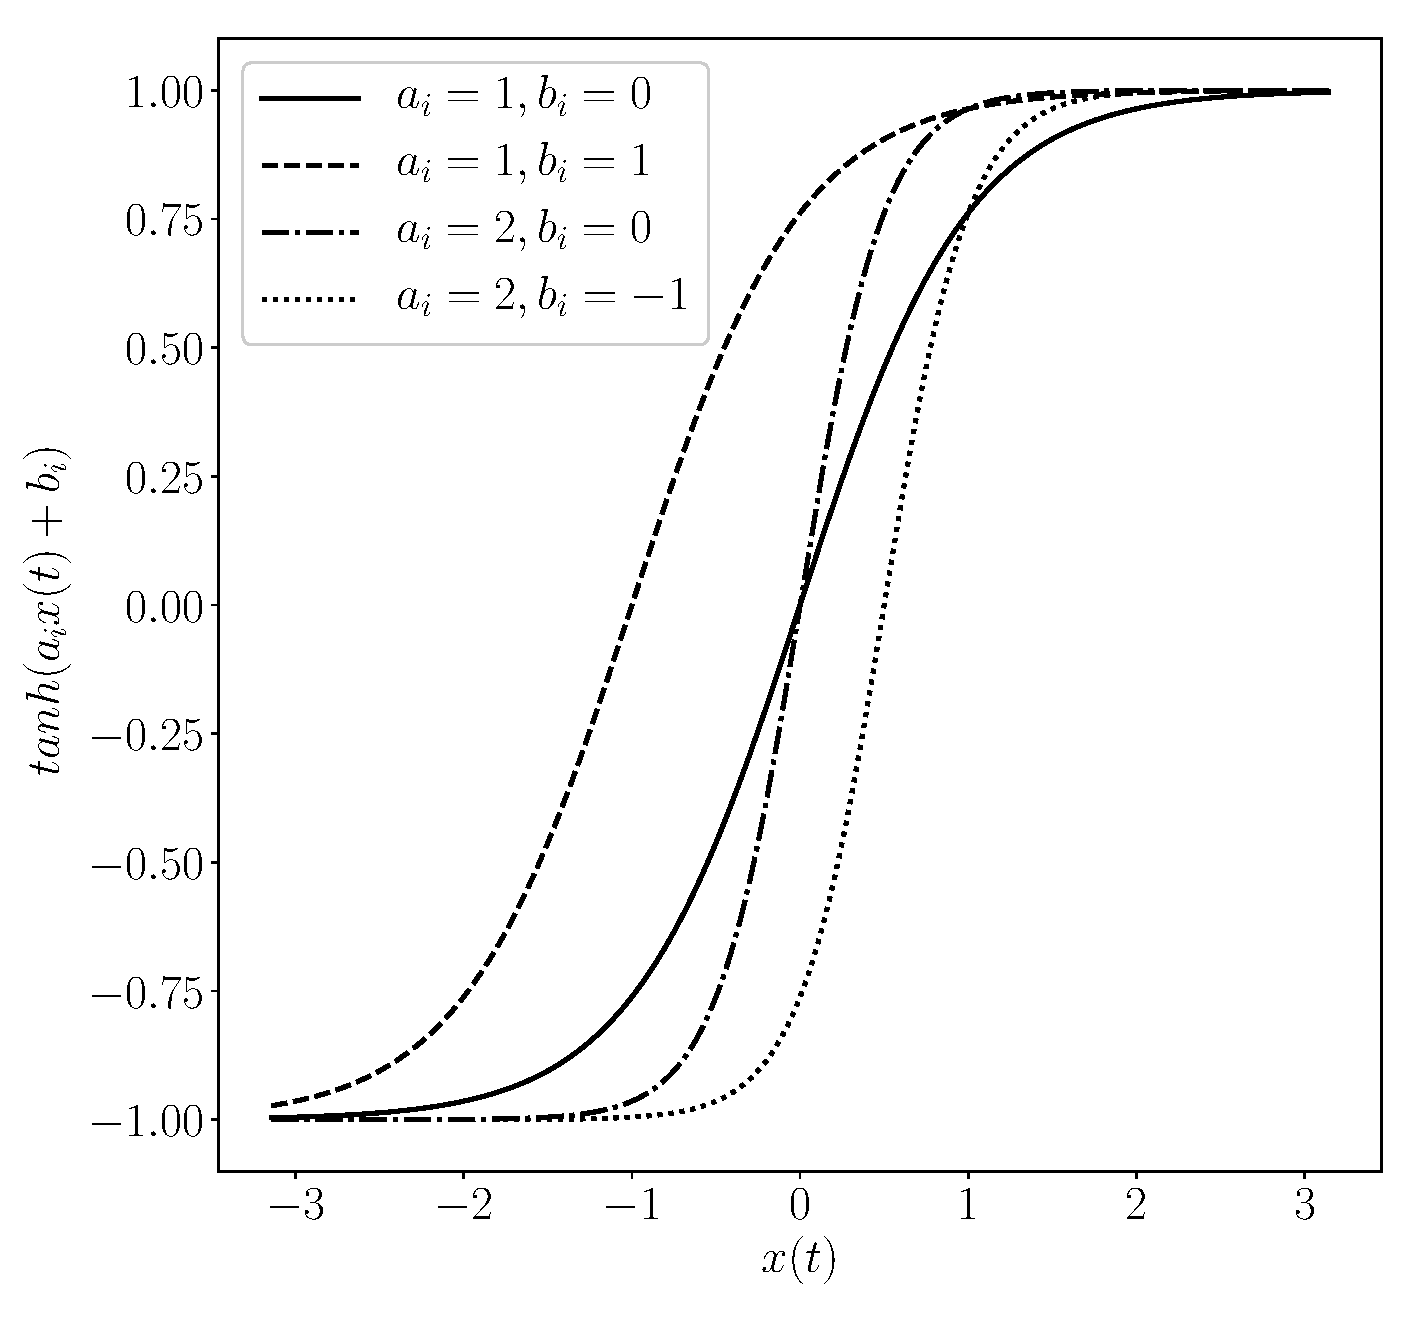
\includegraphics[width=.7\textwidth]{figures/activation_functions}
%    \caption{Shapes of a parametrized tanh activation function.}
%    \label{fig:activation_function}
%\end{figure}
%
%\subsection{Math example}
%The state update of the leaky integrating neuron in figure \ref{fig:leaky_integration} can be formulated as:
%\begin{align}
%    x_i(t+1) &= \lambda_i \cdot \left(W_{i,j} \cdot U_j(t)\right) + (1-\lambda_i) \cdot \theta_i(t)
%    \label{eq:leaky_integration}
%\end{align}
%
%\subsection{Code block example}
%From equation \ref{eq:leaky_integration} the neuron model is implemented using numpy \citep{harris:2020}:
%
%\lstinputlisting[label=py:leaky, language=Python, caption=Python implementation of a single leaky-integrating neuron.]{code/leaky.py}
%
%\subsection{Footnote example}
%The implementation is available on github\footnote{https://github.com/schniewmatz/recurrence}.